
\documentclass[
  bibliography=totoc,     % Literatur im Inhaltsverzeichnis
  captions=tableheading,  % Tabellenüberschriften
  titlepage=firstiscover, % Titelseite ist Deckblatt
  ngerman,
  a4paper
]{article}


\usepackage{lmodern}%Font
\usepackage[T1]{fontenc}
\usepackage[utf8]{inputenc}
\usepackage{scrhack}% Paket float verbessern
\usepackage{longtable}

\usepackage[parfill]{parskip}%linebreaks instead of indention after paragraphs

\usepackage[aux]{rerunfilecheck}% Warnung, falls nochmal kompiliert werden muss
\usepackage{fixltx2e} % provides \textsubscript

\usepackage[shorthands=off,ngerman]{babel}% deutsche Spracheinstellungen

\usepackage{amsmath}% viele Mathe-Symbole
\usepackage{amssymb}
\usepackage{mathtools}
\usepackage{dsfont}

\usepackage{adjustbox}

\usepackage{blindtext}
\usepackage{titlesec}%Page breaks before new sections
\newcommand{\sectionbreak}{\clearpage}

% traditionelle Fonts für Mathematik
%\setmathfont{Latin Modern Math}
%\setmathfont{XITS Math}[range={scr, bfscr}]
%\setmathfont{XITS Math}[range={cal, bfcal}, StylisticSet=1]

% Zahlen und Einheiten
\usepackage[
  locale=DE,                 % deutsche Einstellungen
  separate-uncertainty=true, % immer Fehler mit \pm
  per-mode=reciprocal,       % ^-1 für inverse Einheiten
  output-decimal-marker=.,   % . statt , für Dezimalzahlen
]{siunitx}

% chemische Formeln
\usepackage[
  version=4,
  math-greek=default, % ┐ mit unicode-math zusammenarbeiten
  text-greek=default, % ┘
]{mhchem}

\usepackage[autostyle]{csquotes}% richtige Anführungszeichen
\usepackage{upquote}%straight quotes in verbatim environments
\usepackage{xfrac}% schöne Brüche im Text
\usepackage{grffile}% größere Variation von Dateinamen möglich
\usepackage{booktabs}% schöne Tabellen
\usepackage{microtype}% Verbesserungen am Schriftbild
\setlength{\emergencystretch}{3em}  % prevent overfull lines

% Standardplatzierung für Floats einstellen
\usepackage{float}
\floatplacement{figure}{htbp}
\floatplacement{table}{htbp}
\usepackage[% Floats innerhalb einer Section halten
  section, % Floats innerhalb der Section halten
  below,   % unterhalb der Section aber auf der selben Seite ist ok
]{placeins}

\usepackage{pdflscape}% Seite drehen für breite Tabellen

% Captions schöner machen.
\usepackage[
  labelfont=bf,        % Tabelle x: Abbildung y: ist jetzt fett
  font=small,          % Schrift etwas kleiner als Dokument
  width=0.9\textwidth, % maximale Breite einer Caption schmaler
]{caption}
% subfigure, subtable, subref
\usepackage{subcaption}

\usepackage{graphicx}% Grafiken können eingebunden werden

% Hyperlinks im Dokument
\usepackage[
  unicode,        % Unicode in PDF-Attributen erlauben
  pdfusetitle,    % Titel, Autoren und Datum als PDF-Attribute
  pdfcreator={},  % ┐ PDF-Attribute säubern
  pdfproducer={}, % ┘
]{hyperref}
\hypersetup{breaklinks=true,
            bookmarks=true,
            colorlinks=true,
            citecolor=blue,
            urlcolor=blue,
            linkcolor=magenta,
            pdfborder={0 0 0}
            }
\urlstyle{same}  % don't use monospace font for urls

% Literaturverzeichnis
\usepackage[
  backend=biber,
]{biblatex}
% Quellendatenbank
\addbibresource{lit.bib}
\addbibresource{programme.bib}


% erweiterte Bookmarks im PDF
\usepackage{bookmark}

% Trennung von Wörtern mit Strichen
\usepackage[shortcuts]{extdash}

% --- Macro \xvec
\makeatletter
\newlength\xvec@height%
\newlength\xvec@depth%
\newlength\xvec@width%
\newcommand{\xvec}[2][]{%
  \ifmmode%
    \settoheight{\xvec@height}{$#2$}%
    \settodepth{\xvec@depth}{$#2$}%
    \settowidth{\xvec@width}{$#2$}%
  \else%
    \settoheight{\xvec@height}{#2}%
    \settodepth{\xvec@depth}{#2}%
    \settowidth{\xvec@width}{#2}%
  \fi%
  \def\xvec@arg{#1}%
  \def\xvec@dd{:}%
  \def\xvec@d{.}%
  \raisebox{.2ex}{\raisebox{\xvec@height}{\rlap{%
    \kern.05em%  (Because left edge of drawing is at .05em)
    \begin{tikzpicture}[scale=1]
    \pgfsetroundcap
    \draw (.05em,0)--(\xvec@width-.05em,0);
    \draw (\xvec@width-.05em,0)--(\xvec@width-.15em, .075em);
    \draw (\xvec@width-.05em,0)--(\xvec@width-.15em,-.075em);
    \ifx\xvec@arg\xvec@d%
      \fill(\xvec@width*.45,.5ex) circle (.5pt);%
    \else\ifx\xvec@arg\xvec@dd%
      \fill(\xvec@width*.30,.5ex) circle (.5pt);%
      \fill(\xvec@width*.65,.5ex) circle (.5pt);%
    \fi\fi%
    \end{tikzpicture}%
  }}}%
  #2%
}
\makeatother


%make parantheses scale in math mode
\makeatletter
\def\resetMathstrut@{%
  \setbox\z@\hbox{%
    \mathchardef\@tempa\mathcode`\[\relax
    \def\@tempb##1"##2##3{\the\textfont"##3\char"}%
    \expandafter\@tempb\meaning\@tempa \relax
  }%
  \ht\Mathstrutbox@\ht\z@ \dp\Mathstrutbox@\dp\z@}
\makeatother
\begingroup
  \catcode`(\active \xdef({\left\string(}
  \catcode`)\active \xdef){\right\string)}
\endgroup
\mathcode`(="8000 \mathcode`)="8000

%increase math spacing between lines with fractions
\makeatletter

\newlength\minalignvsep
\def\align@preamble{%
   &\hfil
    \setboxz@h{\@lign$\m@th\displaystyle{##}$}%
    \ifnum\row@>\@ne
    \ifdim\ht\z@>\ht\strutbox@
    \dimen@\ht\z@
    \advance\dimen@\minalignvsep
    \ht\strutbox\dimen@
    \fi\fi
    \strut@
    \ifmeasuring@\savefieldlength@\fi
    \set@field
    \tabskip\z@skip
   &\setboxz@h{\@lign$\m@th\displaystyle{{}##}$}%
    \ifnum\row@>\@ne
    \ifdim\ht\z@>\ht\strutbox@
    \dimen@\ht\z@
    \advance\dimen@\minalignvsep
    \ht\strutbox@\dimen@
    \fi\fi
    \strut@
    \ifmeasuring@\savefieldlength@\fi
    \set@field
    \hfil
    \tabskip\alignsep@
}
\makeatother

\minalignvsep.15em


%align-nummerierung berichtigen
%\numberwithin{equation}{subsection}
%\renewcommand{\theequation}{\thesubsection.\arabic{equation}}

\DeclareMathOperator{\const}{const.}

\author{
  Thea Schneider%
  \texorpdfstring{
    \\
    \href{mailto:thea.schneider@udo.edu}{thea.schneider@udo.edu}
  }{}%
  \texorpdfstring{\and}{, }
  Max Pernklau%
  \texorpdfstring{
    \\
    \href{mailto:max.pernklau@udo.edu}{max.pernklau@udo.edu}
  }{}%
}
%\publishers{TU Dortmund – Fakultät Physik}

\newcommand{\integral}[4]{\int\displaylimits_{#3}^{#4} #1 \, \mathrm{d} #2}
\makeatletter
\newcommand\primitiveinput[1]
{\@@input #1 }
\makeatother

\newcommand*\diff{\mathop{}\!\mathrm{d}}
\newcommand*\Diff[1]{\mathop{}\!\mathrm{d^#1}}
\newcommand{\partialfrac}[2]{\frac{\mathrm{\partial}#1}{\mathrm{\partial}#2}}

\newcommand*\inv[1]{#1^{-1}}

\newcommand{\HRule}{\rule{\linewidth}{0.5mm}}

\begin{document}
\begin{titlepage}
\begin{center}

~\\[1cm]


\textsc{\Large Praktikumsprotokoll des 3.5.2016}\\

% Title
\huge{ \bfseries Millikan-Versuch}\\[1em]


% Author and supervisor
\begin{minipage}{0.4\textwidth}
\begin{flushleft} \large
Thea \textsc{Schneider}\\
thea.schneider@udo.edu
\end{flushleft}
\end{minipage}
\begin{minipage}{0.4\textwidth}
\begin{flushright} \large
Max \textsc{Pernklau}\\
max.pernklau@udo.edu
\end{flushright}
\end{minipage}
%\textsc{\large \newline Durchführung: 15.12.2015} \\

\vfill

{\large \today}

\end{center}
\end{titlepage}


\thispagestyle{empty}
%\tableofcontents
%\newpage

\section{Abstract}
\label{sec:Abstract}
	Durch Bestrahlung verschiedener Spaltöffnungen mit einem Laser wird die Frauenhoferbeugung untersucht.

% this code supresses the \pagebreak that is inserted after each section so that abstract and theory can be on the same page
\begingroup
\renewcommand{\clearpage}{}
\section{Theorie}
\label{sec:Theorie}
\endgroup
\subsection{Licht als Welle}
\label{sec:welle}
Licht hat sowohl die Eigenschaften eines klassischen Teilchens, als auch die einer klassischen Welle -- es unterliegt also dem Prinzip des \emph{Welle-Teilchen-Dualismus} der Quantenphysik. Das sich Licht wie eine Welle verhält, zeigt sich im Experiment besonders anschaulich an seinem Verhalten, wenn es auf eine Öffnung (in einem ansonsten lichtundurchlässigen Hindernissen) trifft, deren Durchmesser innerhalb einiger Größenordnungen der Wellenlänge liegt. Dort tritt Beugung auf und es kann ein für Wellenphänomene typisches Beugungsmuster der Intensität gemessen werden. Die Gesetze der geometrischen Optik erklären dieses Verhalten nicht, da sich Lichtstrahlen in diesem Modell nicht gegenseitig beeinflussen können. Damit wird sowohl Interferrenz, als auch Beugung ausgeschlossen. Von Beugung wird daher gesprochen, wenn die Ausbreitung des Lichtes von diesen Gesetzen abweicht. Auch die Betrachtung von Licht als klassische Welle stellt nur eine Näherung dar, da es sich eigentlich nur mit der Quantenmechanik beschreiben lässt. Breitet sich Licht im Vakuum aus, ist es allerdings möglich den Mittelwert über eine große Anzahl von Lichtquanten zu bilden, wodurch die Näherung des Lichts als Welle anwendbar wird.

Betrachtet man Licht also als Welle, kann das \emph{Huygenssche Prinzip} auf ihr Ausbreitungsverhalten angewendet und als Erklärung für das Auftreten von Beugung verwendet werden. Das Prinzip besagt, dass jeder Punkt einer Wellenfront als Ursprung einer neuen kugelförmigen \emph{Elementarwelle} gleicher Phase interpretiert werden kann. Die Einhüllende aller dieser Elementarwellen bestimmt die Wellenfront für jeden späteren Zeitpunkt. Für die Beschreibung eines bestimmten Punktes der Wellenfront zu einem festgelegten Zeitpunkt müssen daher alle in diesem Zeitpunkt ankommenden Elementarwellen überlagert werden. Die weitere Betrachtung wird nun exemplarisch an einem parallelen Spalt als Öffnung durchgeführt, da mit einem geometrisch einfachem Objekt auch die mathematische Beschreibung vereinfacht wird.

\subsection{Fresnelsche und Fraunhofersche Beugung}

Grundsätzlich kommen zwei in Abbildung~\ref{fig:fresnel} skizzierte Versuchsanordnungen für den Einzelspalt in Frage: Die \emph{Fresnelsche Anordnung}, bei der Lichtquelle und Beobachtungsschirm in endlicher Entfernung zum Spalt aufgebaut sind, zeigt, dass die Strahlenbündel divergieren und somit auch Strahlen (im selben Punkt) interferieren können, die vorher unterschiedlich stark gebeugt wurden (siehe Skizze~\ref{fig:fresnel}~a).

Auf der anderen Seite gibt es die \emph{Fraunhofersche Anordnung}: Hier liegen Lichtquelle und Beobachtungsschirm quasi im Unendlichen, mit der Folge, dass die Strahlen parallel auf den Spalt treffen und somit eine ebene Wellenfront bilden. Als Konsequenz können nur Strahlen im selben Punkt interferieren, die vorher auch unter dem selben Winkel gebeugt wurden (siehe Skizze~\ref{fig:fresnel}~b). Die mathematische Beschreibung der Fraunhoferschen Beugung ist daher einfacher als die der Fresnelschen Beugung. Im Folgenden wird aus diesem Grund nur noch die Fraunhofersche Anordnung betrachtet.

\begin{figure}
  \centering
  \includegraphics[width=0.6\textheight]{../figures/Fresnel.png}
  \caption{Skizze von Fresnelscher (a) und Fraunhoferscher (b) Beugung am Einzelspalt.[Skript V406]}
\label{fig:fresnel}
\end{figure}

\subsection{Beugung am Einzelspalt}
\label{sec:einzel}
Es wird ein Spalt betrachtet, dessen Breite $b$ sehr viel kleiner ist als seine Länge. Das parallel auftreffende Lichtbündel wird dadurch nur in der x-Richtung durch die Breite des Spalts begrenzt. Der Aufbau ist in Abbildung~\ref{fig:spalt} skizziert.

\begin{figure}
  \centering
  \includegraphics[width=0.4\textheight]{../figures/spalt.png}
  \caption{Skizze eines Einzelspaltes bei Fraunhoferscher Beugung.[Skript V406]}
\label{fig:spalt}
\end{figure}

Auf diesen Spalt trifft eine ebene Welle, die durch die Gleichung
\begin{align}
  A(z,t) = A_0 \exp{(i(\omega t - \frac{2 \pi z}{\lambda}))}
  \label{equ:ebeneWelle}
\end{align}
beschrieben wird. Auf Grund des \emph{Huygensschen Prinzips} ist klar, dass die Welle an diesem Spalt gebeugt wird. Um die Feldstärke an einem Punkt bestimmen zu können, muss nach Abschnitt~\ref{sec:welle} über alle Strahlenbündel summiert werden, die unter dem selben Winkel~$\varphi$ abgelenkt werden. Der Abstand dieser Strahlenbündel betrage $x$. Abbildung~\ref{fig:spalt} verdeutlicht, dass der Phasenunterschied zwischen den Strahlenbündeln
\begin{align}
  \delta = \frac{2 \pi s}{\lambda} = \frac{2 \pi x \sin{\varphi}}{\lambda}
  \label{equ:delta}
\end{align}
beträgt. Der Abstand der Strahlenbündel ist allerdings infinitesimal klein, daher muss die Summe in eine Integration über die gesamte Spaltbreite $b$ übergehen. Die Feldstärke der in $\varphi$-Richtung abgelenkten Strahlenbündel kann also durch
\begin{align}
  B(z,t,\varphi) = A_0 \int_0^b \exp{(i(\omega t - \frac{2 \pi z}{\lambda} + \delta))} \mathrm dx
\end{align}
beschrieben werden.
Die Integration sowie einige Umformungsschritte führen für die Feldstärke $B$ auf
\begin{align}
  B(z,t,\varphi) = A_0 \exp{(i(\omega t - \frac{2 \pi z}{\lambda}))} \exp{( \frac{i \pi b \sin{\varphi}}{\lambda})} \frac{\lambda}{\pi \sin{\varphi}} \sin{(\frac{\pi b \sin{\varphi}}{\lambda})} \; .
  \label{equ:B}
\end{align}
Die Orts- und Zeitabhängigkeit der Feldstärke in Ausbreitungsrichtung wird in Gleichung~\eqref{equ:B} durch die erste Exponentialfunktion beschrieben. Die zweite Exponentialfunktion ist ein Phasenfaktor, der von der Richtung abhängig ist. Es handelt sich also lediglich um zwei Phasenfunktionen, die für die Intensitätsmessung keine Bedeutung haben. Die Feldstärke $B$ lässt sich aufgrund der hohen Frequenz des Lichts nicht unmittelbar messen, für eine experimentelle Untersuchung ist daher nur die zeitlich gemittelte Intensität $I(\varphi)$ von Interesse. Sie ist proportional zum Betragsquadrat der Feldstärke
\begin{align}
  I(\varphi) \propto  |B(\varphi)|^2 \; .
\end{align}
Für die Intensität von Licht, das an einem parallelen Einzelspalt gebeugt wurde, folgt daher
\begin{align}
  I(\varphi) = A_0^2 b^2 (\frac{\lambda}{\pi b \sin{\varphi}})^2 \sin^2{(\frac{\pi b \sin{\varphi}}{\lambda})} \; .
  \label{equ:I}
\end{align}
Dabei handelt es sich um einen \emph{Sinus Kardinalis}
\begin{align}
  I(\varphi) \propto \frac{\sin{\chi(\varphi)}}{\chi(\varphi)} \; ,
\end{align}
der die für Beugung typische Intensitätsverteilung liefert (siehe Abbildung~\ref{fig:slit}). Dabei ist $\chi(\varphi) \propto \varphi$.


\subsection{Beugung am Doppelspalt}
Analog zu der Vorgehensweise in Abschnitt~\ref{sec:einzel} kann die Intensitätsverteilung für einen parallelen Doppelspalt berechnet werden. Dafür wird der Doppelspalt als Überlagerung zweier Einzelspalte der Breite $b$ betrachtet, die sich im Abstand $s$ zueinander befinden. Der Aufbau ist in Abbildung~\ref{fig:doppel} skizziert.

\begin{figure}
  \centering
  \includegraphics[width=0.4\textheight]{../figures/doppel.png}
  \caption{Skizze eines Doppelspalts bei Fraunhoferscher Beugung.[Skript V406]}
\label{fig:doppel}
\end{figure}

Die Intensitätsverteilung $I(\varphi)$ ergibt sich damit zu
\begin{align}
  I(\varphi) \propto |B(\varphi)|^2 = 4 \cos^2{\frac{\pi s \sin{\varphi}}{\lambda}}(\frac{\lambda}{\pi b \sin{\varphi}})^2 \sin^2{(\frac{\pi b \sin{\varphi}}{\lambda})} \; .
  \label{equ:I_doppel}
\end{align}
Sie unterscheidet sich von der Intensitätsverteilung des Einzelspaltes nur in dem $\cos^2$-Term. Es entsteht also ein ähnliches Bild für die beiden Intensitätsverteilungen. Durch den $\cos^2$-Term ergeben sich aber mehr Minima und Maxima als beim Einzelspalt, dessen Intensitätsverteilung als die Einhüllende der Doppelspaltintensitätsverteilung dargestellt werden kann (siehe Abbildung~\ref{fig:slit}).

\begin{figure}
  \centering
  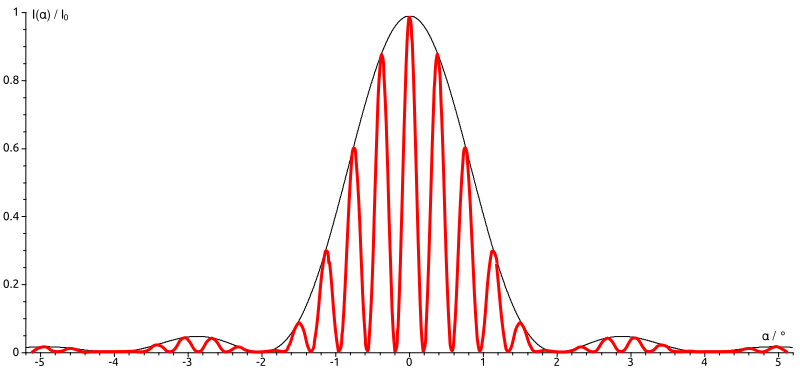
\includegraphics[width=0.4\textheight]{../figures/Slit_double.png}
  \caption{Intensitätsverteilung bei Beugung am Einzelspalt (schwarz) und Doppelspalt (rot). [By Klaus-Dieter Keller]}
\label{fig:slit}
\end{figure}


%This is the end


\newpage

\section{Gaußsche Fehlerrechnung}\label{gausssche-fehlerrechnung}

\subsection{Berechnung der
Standardabweichung}\label{berechnung-der-standardabweichung}

Alle Messwerte sind als empirische Mittelwerte mit ihrer geschätzten
Standardabweichung des Mittelwertes angegeben. Diese unterschätzt die
wahre Standardabweichung, da die Wurzel aus der geschätzten Varianz
gezogen wird. Der arithmetische Mittelwert ist definiert als

\begin{align}
    \bar x = \frac{1}{n} \  \sum_{i=1}^n x_i \  .
    \label{equ:mean}
\end{align}

Die geschätzte Standardabweichung ist gegeben durch

\begin{align}
    s = \sqrt{\frac{1}{n-1} \sum_{i=1}^n (x_i - \bar x)^2}
    \label{equ:s}
\end{align}

mit der geschätzten Standardabweichung des Mittelwertes als

\begin{align}
    \Delta \bar x = \frac{s}{ \sqrt{n} }
    \label{equ:stdofmean}
\end{align}

\subsection{Gaußsche
Fehlerfortpflanzung}\label{gausssche-fehlerfortpflanzung}

Das Berechnen von Funktionen mit fehlerbehafteten Parametern erfolgt
mittels der Gauß'schen Fehlerfortpflanzung

\begin{align}
    \Delta f = \sqrt{ \sum_{i=1}^n \left( \frac{\diff f}{\diff y_i} \right)^2 (\Delta y_i)^2} \qquad \qquad \mathrm{mit} \quad f(y_1, \ldots , y_n)
    \label{equ:gauss}
\end{align}

\newpage
\section{Aufbau und Durchführung}\label{sec:aufbau-und-durchfuehrung}
Der Versuch wird an einem Spektroskop durchgeführt, das wie folgt aufgebaut ist: Eine Lampe wirft durch eine Spaltöffnung einen Lichtstrahl durch ein Linsensystem, sodass ein paralleler Strahl entsteht, der ein drehbar gelagertes Flintglasprisma trifft. Das Licht vom Prisma kann dann durch ein Fernrohr beobachtet werden, an dem eine Winkelskala angebracht ist.

Der Versuch gliedert sich in zwei Abschnitte. Als erstes wird der Winkel~$\varphi$ zwischen den brechenden Prismenoberflächen bestimmt.
Dafür wird eine Kante des Prismas so ausgerichtet und fixiert, dass das Licht der HgCd-Lampe parallel auftrifft und an den beiden angrenzenden Oberflächen reflektiert wird. Der Aufbau ist in Abbildung~\ref{fig:prism} zu sehen.

\begin{figure}
  \centering
  \includegraphics[width=0.4\textheight]{../figures/phi.png}
  \caption{Schematische Darstellung zur Messung des Winkels~$\varphi$ an der brechenden Kante eines Prismas. [Skript V402]}
\label{fig:prism}
\end{figure}

Nun wird das bewegliche Fernrohr so lange gedreht, bis die Spektrallinen des einen reflektierten Strahls genau im Fadenkreuz erscheinen und der Winkel notiert. Genauso verfährt man mit dem zweiten Satz an Spektrallinien. Auf diese Weise erhält man die zwei Winkel $\varphi_{\mathrm l}$ und $\varphi_{\mathrm r}$. Aus geometrischen Überlegungen erhält man für den Winkel~$\varphi$ der Kante
\begin{align}\label{equ:phi}
  \varphi = \frac{1}{2}(\varphi_{\mathrm r} - \varphi_{\mathrm l}) \; .
\end{align}

\par
Als zweites werden die Winkel $\eta_i$ der einzelnen Spektrallinien vermessen, die die Richtungsänderung des einfallenden Strahles charakterisieren.

Dazu wird ein symmetrischer Strahlengang hergestellt (siehe Abbildung~\ref{fig:sympris}). Dazu wird das Prisma so in den Lichtstrahl rotiert, dass Spiegelbild und gebrochenes Bild des Spaltes im Fernrohr unter dem gleichen Winkel erscheinen. Dann wird der Winkel einer Spektrallinie gemessen (bezüglich einer beliebigen, festen Stelle) und das Prisma so um die eigene Achse gedreht, dass spiegelsymmetrisch bezüglich des einfallenden Strahls zum ersten Zustand zu liegen kommt (siehe Abbildung~\ref{fig:spiegel}). Der Winkel, unter dem die gleichfarbige Spektrallinie erscheint wird wieder gemessen und die Differenz zum ersten Winkel $\Delta\Omega$ gebildet. Dadurch ergibt sich der Winkel $\eta$, unter dem der Strahl gebrochen wird zu
\begin{align}\label{equ:eta_}
	\eta = \pi - \Delta\Omega \;.
\end{align}
Dieses Verfahren wird für alle Spektrallinien wiederholt.

Aus den so gemessenen Winkeln ergibt sich mit dem Snelliusschen Brechungsgesetzt folgender Zusammenhang für den Brechungsindex:
\begin{align}\label{equ:brech}
	n = \frac{\sin(\eta/2+\varphi/2)}{\sin(\varphi/2)} \;.
\end{align}

\begin{figure}
  \centering
  \includegraphics[width=0.4\textheight]{../figures/sym.png}
  \caption{Symmetrischer Strahlengang durch ein Prisma. [Skript V402]}
\label{fig:sympris}
\end{figure}

\begin{figure}
  \centering
  \includegraphics[width=0.4\textheight]{../figures/spiegel.png}
  \caption{Prisma wird ``gespiegelt''. [Skript V402]}
\label{fig:spiegel}
\end{figure}
\section{Auswertung}
\label{sec:Auswertung}

% % Examples
% \begin{equation}
%   U(t) = a \sin(b t + c) + d
% \end{equation}
%
% \begin{align}
%   a &= \input{build/a.tex} \\
%   b &= \input{build/b.tex} \\
%   c &= \input{build/c.tex} \\
%   d &= \input{build/d.tex} .
% \end{align}
% Die Messdaten und das Ergebnis des Fits sind in Abbildung~\ref{fig:plot} geplottet.
%
% %Tabelle mit Messdaten
% \begin{table}
%   \centering
%   \caption{Messdaten.}
%   \label{tab:data}
%   \sisetup{parse-numbers=false}
%   \begin{tabular}{
% % format 1.3 bedeutet eine Stelle vorm Komma, 3 danach
%     S[table-format=1.3]
%     S[table-format=-1.2]
%     @{${}\pm{}$}
%     S[table-format=1.2]
%     @{\hspace*{3em}\hspace*{\tabcolsep}}
%     S[table-format=1.3]
%     S[table-format=-1.2]
%     @{${}\pm{}$}
%     S[table-format=1.2]
%   }
%     \toprule
%     {$t \:/\: \si{\milli\second}$} & \multicolumn{2}{c}{$U \:/\: \si{\kilo\volt}$\hspace*{3em}} &
%     {$t \:/\: \si{\milli\second}$} & \multicolumn{2}{c}{$U \:/\: \si{\kilo\volt}$} \\
%     \midrule
%     1.7 & 10 \\
2.3 & 20 \\
3.5 & 30 \\
4.4 & 40 \\

%     \bottomrule
%   \end{tabular}
% \end{table}
%
% % Standard Plot
% \begin{figure}
%   \centering
%   \includegraphics{build/plot.pdf}
%   \caption{Messdaten und Fitergebnis.}
%   \label{fig:plot}
% \end{figure}
%
% 2x2 Plot
% \begin{figure*}
%     \centering
%     \begin{subfigure}[b]{0.475\textwidth}
%         \centering
%         \includegraphics[width=\textwidth]{Abbildungen/Schaltung1.pdf}
%         \caption[]%
%         {{\small Schaltung 1.}}
%         \label{fig:Schaltung1}
%     \end{subfigure}
%     \hfill
%     \begin{subfigure}[b]{0.475\textwidth}
%         \centering
%         \includegraphics[width=\textwidth]{Abbildungen/Schaltung2.pdf}
%         \caption[]%
%         {{\small Schaltung 2.}}
%         \label{fig:Schaltung2}
%     \end{subfigure}
%     \vskip\baselineskip
%     \begin{subfigure}[b]{0.475\textwidth}
%         \centering
%         \includegraphics[width=\textwidth]{Abbildungen/Schaltung4.pdf}    % Zahlen vertauscht ... -.-
%         \caption[]%
%         {{\small Schaltung 3.}}
%         \label{fig:Schaltung3}
%     \end{subfigure}
%     \quad
%     \begin{subfigure}[b]{0.475\textwidth}
%         \centering
%         \includegraphics[width=\textwidth]{Abbildungen/Schaltung3.pdf}
%         \caption[]%
%         {{\small Schaltung 4.}}
%         \label{fig:Schaltung4}
%     \end{subfigure}
%     \caption[]
%     {Ersatzschaltbilder der verschiedenen Teilaufgaben.}
%     \label{fig:Schaltungen}
% \end{figure*}

\section{Diskussion}
\label{sec:Diskussion}
  Die Mikroskopdaten sind entsprechend der Messmethode ungenau, aber eine notwendige Orientierung zum finden der Fitparameter.
  Der Rahmen auf dem Bildschirm war recht dick und ließ keine genaue Messung zu. Zudem ist der digitale Zoom des
  Mikroskops nur sehr grob einstellbar.

  Das Fitten der Daten gestaltete sich äußerst aufwendig; der zu fittende Sinus Cardinalis stellt ein großes Problem dar,
	da die zu minimierende Funktion der Summe der Abweichungsquadrate stark oszilliert und auf kleinen Bereichen viele
	lokale Minima besitzt, was eine Verwendung von Gradient-orientierten Fittern beinahe ausschließt, da diese hier
	nicht robust genug sind.
	Die Autoren benutzten schlussendlich eine modifizierte Version des \emph{Simplex}-Algorithmus in Tandem mit
	\emph{Mathematicas NonlinearModelFit}, die in der Kürze der Zeit ein noch annehmbares Ergebnis lieferten. Dabei wurde
	insbesondere darauf geachtet, die Frequenz (des Sinus Cardinalis) der Messdaten möglichst gut zu fitten, da diese für die Spaltbreite bestimmend
	ist.

	Die Messdaten zu den ersten drei Spalten sind gut genug, um die Spaltbreite zu bestimmen. Sie haben etwa 25~\% Abweichung
	zu den mikroskopierten Werten. Es gibt keine Anhaltspunkte, welches der beiden Messverfahren genauer ist.

	Die Messdaten des Doppelspalts weichen zu stark von dem nach der Theorie erwarteten Muster ab. Der hindurchgelegte Fit
	weicht zu stark ab, um aussagekräftig zu sein. Die Messdaten haben mehr den Charakter zwei weit voneinander entfernter
	Einzelspalte. Schlussendlich konnte nicht erklärt werden, warum der zu erwartende Peak in der Mitte des Diagramms ausbleibt.


\subsection{Messdaten} % (fold)
\label{sub:messdaten}

\begin{table}
\footnotesize
	\centering
  \caption{Messdaten zu Spalt 1.}
  \label{tab:fit}
  \begin{adjustbox}{center}
		\tabcolsep=0.11cm
  \begin{tabular}{
      S
      S
      S}
   \toprule
   \multicolumn{1}{c}{Winkel in mrad} &
   \multicolumn{1}{c}{Strom in \si{\mu\ampere}} &
   \multicolumn{1}{c}{Strom $\sigma$ in \si{\mu\ampere}} \\
   \midrule
      \primitiveinput{../table/single_slit1.tex}
   \bottomrule
  \end{tabular}
  \end{adjustbox}
\end{table}

\begin{table}
\footnotesize
	\centering
  \caption{Messdaten zu Spalt 2.}
  \label{tab:fit}
  \begin{adjustbox}{center}
		\tabcolsep=0.11cm
  \begin{tabular}{
      S
      S
      S}
   \toprule
   \multicolumn{1}{c}{Winkel in mrad} &
   \multicolumn{1}{c}{Strom in \si{\mu\ampere}} &
   \multicolumn{1}{c}{Strom $\sigma$ in \si{\mu\ampere}} \\
   \midrule
      \primitiveinput{../table/single_slit2.tex}
   \bottomrule
  \end{tabular}
  \end{adjustbox}
\end{table}

\begin{table}
\footnotesize
	\centering
  \caption{Messdaten zu Spalt 3.}
  \label{tab:fit}
  \begin{adjustbox}{center}
		\tabcolsep=0.11cm
  \begin{tabular}{
      S
      S
      S}
   \toprule
   \multicolumn{1}{c}{Winkel in mrad} &
   \multicolumn{1}{c}{Strom in \si{\mu\ampere}} &
   \multicolumn{1}{c}{Strom $\sigma$ in \si{\mu\ampere}} \\
   \midrule
      \primitiveinput{../table/single_slit3.tex}
   \bottomrule
  \end{tabular}
  \end{adjustbox}
\end{table}

\begin{table}
\footnotesize
	\centering
  \caption{Messdaten zu Spalt 4 (Doppelspalt).}
  \label{tab:fit}
  \begin{adjustbox}{center}
		\tabcolsep=0.11cm
  \begin{tabular}{
      S
      S
      S}
   \toprule
   \multicolumn{1}{c}{Winkel in mrad} &
   \multicolumn{1}{c}{Strom in \si{\mu\ampere}} &
   \multicolumn{1}{c}{Strom $\sigma$ in \si{\mu\ampere}} \\
   \midrule
      \primitiveinput{../table/single_slit4.tex}
   \bottomrule
  \end{tabular}
  \end{adjustbox}
\end{table}


% subsection messdaten (end)

\newpage
\section{Literaturangabe}
\label{sec:Literatur}

Bilder und Daten aus dem Skript zu \emph{Beugung am Spalt}, Versuch 406, TU Dortmund, abrufbar auf:\\
\url{http://129.217.224.2/HOMEPrismadispersionPAGE/PHYSIKER/BACHELOR/AP/SKRIPT/V406.pdf}\\(Stand 30.04.16)\par

Bild zu \emph{Intensitätsverteilung am Doppelspalt}, By Klaus-Dieter Keller - Own work, created with SciDAVisThis vector image was created with Inkscape., CC BY 3.0,
abrufbar auf: \\
\url{https://commons.wikimedia.org/w/index.php?curid=24952635 }\\ (Stand 30.04.16)



%\printbibliography

\end{document}
